% =============================================================
%  Chapter -- Station calculation
%  The chapter heading and introduction; the content is one file per
%  subsection, \input below in reading order:
%    ac-side.tex      PCC, AC line, converter transformer
%    dc-side.tex      DC reactor and station DC terminal
%    procedures.tex   power given at the PCC or at the DC terminal,
%                     station totals and checks
%    example.tex      worked example (Tables chain, losses, procedures;
%                     Figure single-line with the results)
%  Figures and tables: fig/, generated by fig/station_example.py from
%  tools/example_data.py; the single-line diagram fig/loadflow_station.pdf
%  is cast by Glyphwright from examples/sld/loadflow_station.yaml and
%  filled with the results by StationService.single_line.
%  Sources: [1] hvdc_lf, src/hvdc_lf/station, components/ac_network,
%  ac_line, transformer, reactor.
% =============================================================
\section{Station Calculation}
\label{sec:station}

A station is calculated element by element from the AC grid to its DC terminal:

\begin{center}
  PCC $\rightarrow$ AC line $\rightarrow$ transformer $\rightarrow$ arm reactors $\rightarrow$ converter
  $\rightarrow$ DC reactors $\rightarrow$ station DC terminal
\end{center}

The voltage, frequency, reactive power and tap are given at the PCC, the DC voltage $U_{dpe}$ at the station DC
terminal (the DC line interface, after the DC reactor), and the active power either at the PCC or at the station
DC terminal. Each element takes the output of the previous one as its input. The AC line and the DC reactor are
optional; the transformer and the converter are calculated per converter, with $1/n_{conv}$ of the station power.
The converter is described in Section~\ref{sec:converter}; this chapter gives the other elements, the solution
procedures and a worked example.

\subsection{AC Side}
\label{sec:station-ac}

\subsubsection{AC network at the PCC}

The voltage is defined at the PCC, so the AC network behind it needs no impedance. The PCC holds the boundary
values $U_{pcc}$, $f$, $P_{pcc}$ and $Q_{pcc}$ of the operating point; its current is
\begin{equation}
  I_{pcc} = \frac{\left| \underline{S}_{pcc} \right|}{\sqrt{3} \cdot U_{pcc}} ,
  \qquad \underline{S}_{pcc} = P_{pcc} + \mathrm{j} \cdot Q_{pcc} .
\end{equation}
The PCC voltage is reported in per unit of the nominal voltage and checked against the voltage band of the network.

\subsubsection{AC line}

The AC line between the PCC and the transformer is a nominal $\pi$ section: series impedance $\underline{Z}$ and
half the line capacitance at each end. With $n_c$ circuits in parallel, $n_b$ sub-conductors per phase of an OHL
and $n_k$ cables per phase of a cable line,
\begin{equation}
  \underline{Z} = \left( \frac{R'}{n_b} + \mathrm{j} \cdot X' \cdot \frac{f}{f_r} \right) \cdot \frac{l}{n_k \cdot n_c} ,
  \qquad B = \omega \cdot C' \cdot l \cdot n_k \cdot n_c .
\end{equation}
The charging power of one end and the absorbed power of a shunt reactor at that end are
\begin{equation}
  Q_c(U) = \frac{U^2 \cdot B}{2} , \qquad Q_r(U) = Q_{r\_n} \cdot \left( \frac{U}{U_n} \right)^2 .
\end{equation}
The calculation starts at the PCC, where voltage and power are known, and ends at the station end:
\begin{align}
  \underline{S}_{ser} &= \underline{S}_{pcc} - \mathrm{j} \cdot \left( Q_c(U_{pcc}) - Q_{r\_pcc} \right) , \\
  \underline{I} &= \left( \frac{\underline{S}_{ser}}{\sqrt{3} \cdot U_{pcc}} \right)^{*} , \\
  \underline{U}_{st} &= U_{pcc} + \sqrt{3} \cdot \underline{Z} \cdot \underline{I} , \\
  \underline{S}_{st} &= \sqrt{3} \cdot \underline{U}_{st} \cdot \underline{I}^{*}
                        - \mathrm{j} \cdot \left( Q_c(|\underline{U}_{st}|) - Q_{r\_st} \right) .
\end{align}
$\underline{I}$ is the series current towards the grid, with the PCC voltage as phase reference. The losses are
$P_{loss\_line} = P_{st} - P_{pcc}$; the loading is the highest of the series, PCC and station-end currents in
per cent of the rated current of all circuits. The method \texttt{series} omits the capacitance.

\subsubsection{Converter transformer}

The transformer model (method \texttt{simplified}) has the no-load branch on the line side, an ideal ratio with the
tap changer and the short-circuit impedance on the valve side. Referred to the valve side,
\begin{equation}
  Z_{base} = \frac{U_{r\_valve}^2}{S_r} , \quad
  Z_k = \frac{u_k}{100} \cdot Z_{base} , \quad
  R = \frac{P_{cu}}{S_r} \cdot Z_{base} , \quad
  X = \sqrt{Z_k^2 - R^2} \cdot \frac{f}{f_r} .
\end{equation}
The ratio $n = U_{line} / U_{valve}$ with the tap position $t$ and the step $\Delta_t$ in per cent is
\begin{equation}
  n = \frac{U_{r\_line} \cdot (1 + t \cdot \Delta_t / 100)}{U_{r\_valve}} \quad \text{(tap on the line side)} ,
  \qquad
  n = \frac{U_{r\_line}}{U_{r\_valve} \cdot (1 + t \cdot \Delta_t / 100)} \quad \text{(valve side)} .
\end{equation}
The no-load power scales with the square of the line voltage,
$\underline{S}_0 = \left( P_{fe} + \mathrm{j} \cdot \tfrac{i_0}{100} \cdot S_r \right) \cdot (U_{line} / U_{r\_line})^2$.
The auxiliary power of the station $P_{aux}$ (cooling, control, building services) is part of the operating point
and a constant load at the line side, $1/n_{conv}$ of it per transformer. The valve-side quantities follow from the
line side:
\begin{align}
  \underline{S}_{ser} &= \underline{S}_{line} + P_{aux} / n_{conv} + \underline{S}_0 , \qquad
  U_1' = U_{line} / n , \\
  \underline{I}_2 &= \left( \frac{\underline{S}_{ser}}{\sqrt{3} \cdot U_1'} \right)^{*} , \qquad
  \underline{U}_2 = U_1' + \sqrt{3} \cdot \underline{Z} \cdot \underline{I}_2 , \qquad
  \underline{S}_{valve} = \sqrt{3} \cdot \underline{U}_2 \cdot \underline{I}_2^{*} .
\end{align}
The losses are $P_{loss\_tr} = P_{valve} - P_{line} - P_{aux} / n_{conv}$, the loading is
$\left| \underline{S}_{line} + P_{aux}/n_{conv} \right| / S_r$. A tap outside its range is rejected; a tap at the end
of the range and a loading above 100\,\% are warnings. The method \texttt{ideal} keeps the ratio and the auxiliary
power and omits losses and voltage drop.

\subsection{DC Side}
\label{sec:station-dc}

The DC voltage $U_{dpe}$ is given at the station DC terminal, the interface to the DC line. The DC reactor of each
pole lies between the converter terminal and the station DC terminal. With $R_{dcr}$ the resistance of one DC reactor
and $I_d$ the DC current of a pole,
\begin{equation}
  U_{dpe\_conv} = U_{dpe} + R_{dcr} \cdot I_d \quad \text{(rectifier)} , \qquad
  U_{dpe\_conv} = U_{dpe} - R_{dcr} \cdot I_d \quad \text{(inverter)} ,
\end{equation}
since the DC current flows out of the rectifier and into the inverter. The converter sees the voltage
$U_{dc} = k \cdot U_{dpe\_conv}$ across its terminals. The power at the station DC terminal, all poles, is
\begin{equation}
  P_{dc\_terminal} = n_{conv} \cdot P_{dc\_cv} + 2 \cdot R_{dcr} \cdot I_d^2 ,
\end{equation}
with $P_{dc\_cv}$ the DC power of one converter in the sign convention of Section~\ref{sec:conventions}. In steady
state the inductance of the DC reactor has no effect. Without a DC reactor, $U_{dpe\_conv} = U_{dpe}$.

\subsection{Solution Procedures}
\label{sec:station-procedures}

\subsubsection{Active power given at the PCC}

With $P_{pcc}$ given, the AC network, the AC line, the transformer and the converter are calculated once in this
order. The converter needs its DC voltage, which depends on the DC current through the DC reactor
(Section~\ref{sec:station-dc}), and the DC current follows from the converter. This loop is solved by a fixed-point
iteration on $U_{dpe\_conv}$:
\begin{enumerate}
  \item start with $U_{dpe\_conv} = U_{dpe}$;
  \item calculate the chain with $U_{dc} = k \cdot U_{dpe\_conv}$, giving $I_d$;
  \item update $U_{dpe\_conv} = U_{dpe} \pm R_{dcr} \cdot I_d$ and repeat from step 2 until the change is below
        $10^{-10}$\,kV.
\end{enumerate}
Without a DC reactor one pass is enough. The losses of the converter depend on its DC current
$I_{dc} = (P_{ac} + P_{loss\_cv}) / U_{dc}$; inside the converter they are found by a fixed-point iteration as
well (Section~\ref{sec:converter-losses}).

\subsubsection{Active power given at the DC terminal}

With $P_{dc}$ given at the station DC terminal (all poles), the DC side is known directly:
\begin{equation}
  I_d = \frac{|P_{dc}|}{n_{conv} \cdot k \cdot U_{dpe}} , \qquad
  U_{dpe\_conv} = U_{dpe} \pm R_{dcr} \cdot I_d , \qquad
  P_{dc\_cv}^{target} = \mp k \cdot U_{dpe\_conv} \cdot I_d ,
\end{equation}
upper signs for a rectifier ($P_{dc} < 0$). The PCC power is the root of
\begin{equation}
  F(P_{pcc}) = P_{dc\_cv}(P_{pcc}) - P_{dc\_cv}^{target} ,
\end{equation}
where $P_{dc\_cv}(P_{pcc})$ is the converter DC power from the AC chain at the fixed converter voltage. The root is
found by the secant method, starting from $P_{pcc} = n_{conv} \cdot P_{dc\_cv}^{target}$ and 1.01 times that value,
with the tolerance $10^{-9}$\,MW and at most 50 iterations.

\subsubsection{Station totals and checks}

The station losses are
\begin{equation}
  P_{loss\_st} = n_{conv} \cdot \left( P_{loss\_tr} + P_{aux}/n_{conv} + P_{loss\_cv} \right)
                 + 2 \cdot R_{dcr} \cdot I_d^2 + P_{loss\_line} ,
\end{equation}
and the efficiency is the output power divided by the input power: $|P_{dc}| / |P_{pcc}|$ for a rectifier,
$P_{pcc} / P_{dc}$ for an inverter. The result carries the operation that follows from the sign of the given power
and warnings for a PCC voltage outside its band, an AC line or transformer loading above 100\,\% and every exceeded
limit of the converter. A rectifier whose converter would not deliver DC power, or the reverse for an inverter, is
rejected.

\subsection{Worked Example}
\label{sec:station-example}

Table~\ref{tab:station-chain} gives the chain of the example station (Section~\ref{sec:example-data}) at
$P_{pcc} = -1000$\,MW: voltage, active and reactive power and current at the output of each element and the losses
of that element. The station delivers $P_{dc} = \exPdc$\,MW at its DC terminal with $I_d = \exId$\,kA; the losses
are $\exLoss$\,MW and the efficiency is $\exEta$\,\%. The modulation index is $m = \exM$ and the converter DC voltage
$U_{dpe\_conv} = \exUconv$\,kV. Table~\ref{tab:station-losses} splits the losses by element, and
Figure~\ref{fig:station-sld} shows the same results in the single-line diagram of the station.

\begin{table}[!ht]
  \centering
  \small
  \begin{tabularx}{\linewidth}{@{}>{\raggedright\arraybackslash}X r r r r r@{}}
    \toprule
    \textbf{Element (output)} & \multicolumn{1}{c}{\textbf{$U$ [kV]}} & \multicolumn{1}{c}{\textbf{$P$ [MW]}}
      & \multicolumn{1}{c}{\textbf{$Q$ [Mvar]}} & \multicolumn{1}{c}{\textbf{$I$ [kA]}}
      & \multicolumn{1}{c}{\textbf{$P_{loss}$ [MW]}} \\
    \midrule
    \tablerows{station/fig/chain_table}
    \bottomrule
  \end{tabularx}
  \caption{Station chain of the example at $P_{pcc} = -1000$\,MW, $U_{dpe} = 400$\,kV, $P_{aux} = 500$\,kW. AC rows:
           voltage line-to-line, current per converter on the valve side; arm reactor row: internal converter
           voltage and arm current (RMS); DC rows: voltage pole-to-ground, DC current, converter row with the sign of
           the convention}
  \label{tab:station-chain}
\end{table}

\begin{table}[!ht]
  \centering
  \small
  \begin{tabular}{@{}l r r@{}}
    \toprule
    \textbf{Part} & \multicolumn{1}{c}{\textbf{MW}} & \multicolumn{1}{c}{\textbf{\% of $|P_{pcc}|$}} \\
    \midrule
    \tablerows{station/fig/losses_table}
    \bottomrule
  \end{tabular}
  \caption{Loss breakdown of the example station}
  \label{tab:station-losses}
\end{table}

\begin{figure}[!ht]
  \centering
  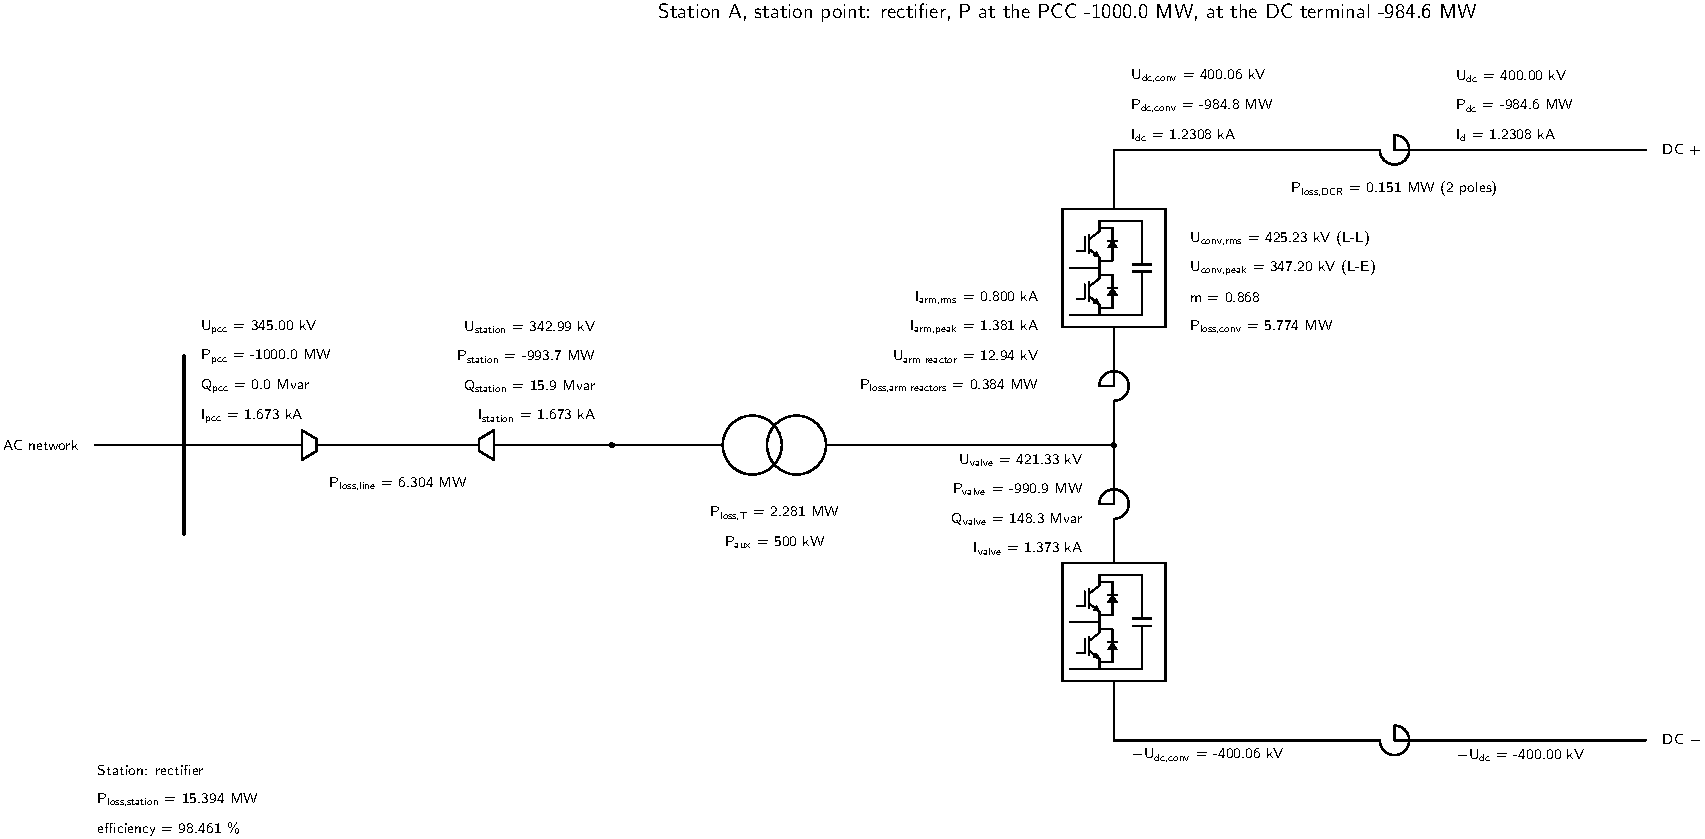
\includegraphics[width=\linewidth]{station/fig/loadflow_station.pdf}
  \caption{Single-line diagram of the example station with the results of Table~\ref{tab:station-chain}}
  \label{fig:station-sld}
\end{figure}

Table~\ref{tab:station-procedures} compares the two solution procedures of Section~\ref{sec:station-procedures}.
The DC power of the first row, given at the DC terminal, reproduces the PCC power after 4 secant iterations. The
third row is an inverter with $P_{dc} = 990$\,MW.

\begin{table}[!ht]
  \centering
  \small
  \begin{tabular}{@{}l r r r r r@{}}
    \toprule
    \textbf{Power given} & \multicolumn{1}{c}{\textbf{$P_{pcc}$ [MW]}} & \multicolumn{1}{c}{\textbf{$P_{dc}$ [MW]}}
      & \multicolumn{1}{c}{\textbf{$I_d$ [kA]}} & \multicolumn{1}{c}{\textbf{$U_{dpe\_conv}$ [kV]}}
      & \multicolumn{1}{c}{\textbf{Iterations}} \\
    \midrule
    \tablerows{station/fig/procedures_table}
    \bottomrule
  \end{tabular}
  \caption{Active power given at the PCC and at the station DC terminal; iterations of the secant method}
  \label{tab:station-procedures}
\end{table}
\FloatBarrier

